\documentclass[preprint]{sigplanconf}
\usepackage{xspace,url,subfigure,framed,amssymb,
            amsmath,mathpartir,hyperref,
            stmaryrd, graphicx, fancyvrb, stmaryrd % double brackets llbracket
}

\usepackage[T1]{fontenc}
\usepackage{beramono}
\usepackage{listings}
\usepackage[usenames,dvipsnames]{xcolor}

\lstdefinelanguage{Julia}%
  {morekeywords={abstract,break,case,catch,const,continue,do,else,elseif,%
      end,export,false,for,function,immutable,import,importall,if,in,%
      macro,module,otherwise,quote,return,switch,true,try,type,typealias,%
      using,while},%
   sensitive=true,%
   morecomment=[l]\#,%
   morecomment=[n]{\#=}{=\#},%
   morestring=[s]{"}{"},%
   morestring=[m]{'}{'},%
}[keywords,comments,strings]%

\lstset{%\lstinputlisting[language=Octave]{BitXorMatrix.m}
    language         = Julia,
    basicstyle       = \small\ttfamily,
    keywordstyle     = \bfseries\color{blue},
    stringstyle      = \color{magenta},
    commentstyle     = \color{ForestGreen},
    showstringspaces = false,
    stepnumber=1,
    numbers=left
}

\newcommand{\rn}[1]{#1}
\newcommand{\doi}[1]{doi:~\href{http://dx.doi.org/#1}{\Hurl{#1}}}

\newcommand{\xt}[1]{\texttt{#1}}

\newcommand{\OK}[1]{#1\;\text{OK}}
\newcommand{\abstype}[2]{\xt{abstract}~#1 <: #2}
\newcommand{\oftype}[2]{#1\,::\,#2}
\newcommand{\m}[2]{{#1}(#2)}
\newcommand{\contype}[2]{\xt{type}~#1 <: #2}
\newcommand{\any}{\xt{any}}

\newcommand{\exact}[1]{{\llbracket #1 \rrbracket_{\xt{exact}}}}
\newcommand{\usable}[1]{{\llbracket #1 \rrbracket_{\xt{}}}}
\renewcommand{\ldots}{...}


\conferenceinfo{NOOL '16}{Month d--d, 20yy, City, ST, Country} 
\copyrightyear{20yy}
\copyrightdata{978-1-nnnn-nnnn-n/yy/mm}
\copyrightdoi{nnnnnnn.nnnnnnn}
\begin{document}
\title{Bottom Up Objects: Static Typing Without Types} 
\authorinfo{Benjamin Chung \and Paley Li \and Jan Vitek}{Northeastern University}{bchung@ccs.neu.edu \and \{pa.li,j.vitek\}@neu.edu} % Annon : Benjamin Chung, Jan Vitek}{Northeastern University}{}
\maketitle
% We should probably have some more introductory/motivational material herezies

\begin{figure}
\centering
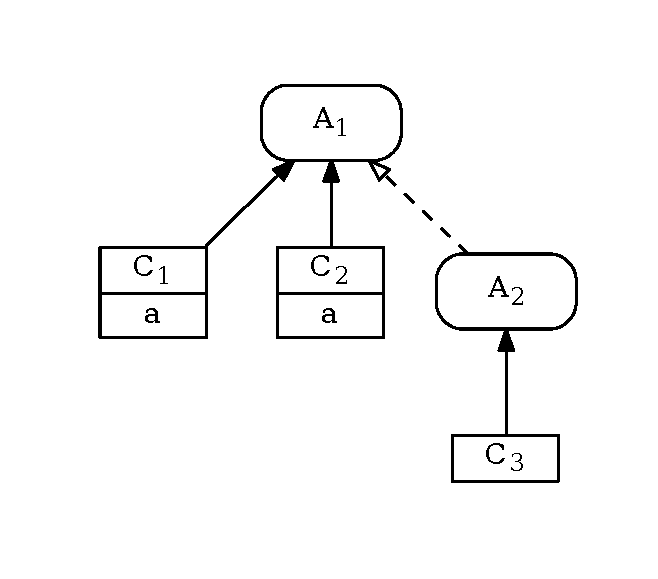
\includegraphics[scale=.6]{example2.pdf}
\caption{LALALALA}
\label{fig:algo}
\end{figure}

\section{Introduction}

Traditional typed object-oriented languages have a series of
common idioms: single dispatch, to figure out which method
to use in which situation, interfaces, to abstract over 
common means of access, and the means to statically
ensure that those interfaces are adhered to.

These practices are perfectly suitable for many contexts,
as is demonstrated by the success of langauges that have 
these features, but are not universally applicable, and
other languages that do not have any of these features
can use the object abstraction while retaining static 
safety.

In this paper, we will be talking about the Julia
programming language. Julia was originally designed
as a scientific computing language, in the vein of 
R or Matlab, and has a number of features designed
to support numeric computation and other tasks common
in scientific work.

Julia departs from the object oriented norms in all 
three ways:
\begin{itemize}
\item \emph{Multiple dispatch},using runtime type
information to dispatch to the ``most specific'' method.
\item \emph{No explicit classes or interfaces} - 
but Julia does have subtyping, over structs (which are leaves in
the inheritance heirarchy, and act as records) and for 
abstract types, which are empty labels that allow the 
construction of heirarchies of types.
\item \emph{Dynamic typing}. Julia is dynamically typed,
but most Julia programs are heavily type annotated to leverage
Julia's multiple dispatch.
\end{itemize}

For our purposes, the second deviation is the most interesting, as in Julia
abstract types, the only types that can be subtyped from, cannot define an
interface that can be safely consumed. An example of a Julia inheritance hierarchy
is shown in figure~\ref{fig:algo}, where $A_1$ and $A_2$ are abstract types and
$C_1$ through $C_3$ are structs or concrete types.

Julia programs do have a notion of a functional interface, however, but it does
not arise from the language itself. Julia programmers leverage the third property
- dynamic typing - to perform operations on an abstract type that cannot be supported
by the type itself, following interfaces defined by convention, an idiom that is suggested
by the language documentation~\cite{juliadocu}.

The problem with this approach arises in situations like the one shown in figure~\ref{code:broken}.
Here, we expect the function \xt{example} to work on anything of type \xt{A1}, which we then
try and call in \xt{problem}. This works fine if we just call it with a \xt{C1}, which has
a function \xt{example} defined for it, but if we call it with a \xt{C3} as seen on line 12,
then the pictured error message is produced, as \xt{C3} has no method \xt{example}.

We propose that we can check these conventions statically, using the type information that
is already in the program. Our system structurally infers the interfaces of abstract types
from concrete implementations, then checks that those interfaces are used correctly in client
code. Our goal is to be able to detect errors like those encountered in figure~\ref{code:broken}
before the program is executed, providing programmers with assurance that invocations will succeed.


\begin{figure}

\lstinputlisting[language=Julia]{broken.jl}
\begin{Verbatim}[fontsize=\small]
ERROR: MethodError: no method matching example(::C3)
Closest candidates are:
  example(::C1)
\end{Verbatim}
\caption{LALALA}
\label{code:broken}
\end{figure}

 \newpage

\begin{figure}
\begin{align*}
t ::=~& n ~|~ \any\\
d ::=~& \abstype{n}{t} ~|~ \contype{n}{t} \\
  & |~ \m{m}{\oftype{a}{t}, ~\ldots} = e\\
e ::=~& x ~|~ \xt{new} ~ n(e,~\ldots) ~|~ m(e,~\ldots) \\
\end{align*}
\caption{LALALA}
\end{figure}

% \usable{A} \equiv \exact{A} \cup 
%	\bigcap_{C <: A} \usable{C} 
%	\bigcap_{A' <: A} \usable{A'}

\begin{figure}
\begin{mathpar}
\inferrule*[lab={\tiny TAbsSelf}]{ }{ \m{m}{\ldots, \oftype{a}{A}, \ldots} \in \usable{A} }

\inferrule*[lab={\tiny TConSelf}]{ }{ \m{m}{\ldots, \oftype{a}{C}, \ldots} \in \usable{C} }

\inferrule*[lab={\tiny TAbsChild}]{\forall C <: A, \m{m}{\ldots} \in \usable{C}\\ \forall A' <: A, \m{m}{\ldots} \in \usable{A'}}{ \m{m}{\ldots} \in \usable{A} }

\end{mathpar}
\caption{LALALA}
\end{figure}
\bibliographystyle{plain}
\bibliography{main}
\end{document}